\documentclass[twoside,11pt]{article}

% Any additional packages needed should be included after jmlr2e.
% Note that jmlr2e.sty includes epsfig, amssymb, natbib and graphicx,
% and defines many common macros, such as 'proof' and 'example'.
%
% It also sets the bibliographystyle to plainnat; for more information on
% natbib citation styles, see the natbib documentation, a copy of which
% is archived at http://www.jmlr.org/format/natbib.pdf

\usepackage{jmlr2e}
\usepackage{float}
\usepackage{hyperref}
\usepackage{parskip}
\usepackage{biblatex}
\addbibresource{proposal.bib}
\usepackage[letterpaper, portrait, margin=1in]{geometry}
\usepackage{graphicx}


% Definitions of handy macros can go here
\newcommand{\dataset}{{\cal D}}
\newcommand{\fracpartial}[2]{\frac{\partial #1}{\partial  #2}}
% Heading arguments are {volume}{year}{pages}{submitted}{published}{author-full-names}

% Short headings should be running head and authors last names
\ShortHeadings{Predicting EMS Response Time}{Acharya}
\firstpageno{1}

\begin{document}

\title{90-904: Predicting EMS Response Times in New York City}

\author{\name Prithvi S. Acharya \email PACHARYA/acharyap@cmu.edu \\
       \addr Engineering and Public Policy\\
       Carnegie Mellon University\\
       Pittsburgh, PA, United States \\
       }
       
\maketitle
\begin{abstract}
    Our study shows that the best indicator of EMS response time in New York City was the travel time, and that the response time appears to not depend very heavily on the type of call, the time of day, or demographic/location data. Further, in spite of using two ensemble models in addition to linear regression models, we were unable to build a compelling machine learning model to predict EMS response time; of the models we tested, a Random Forest appeared to have the best performance. Further study to use real-time traffic and ambulance availability data to predict ambulance travel time is critical to predicting EMS response time.
\end{abstract}
\section{Introduction}
In this project, we build and test multiple machine learning models to predict the Emergency Medical Service (EMS) Response Time (i.e., the time between when an emergency call was received, to when the first EMS personnel arrive on the site of the incident) in New York City, based on past EMS call data available from the City of New York. By comparing the models' prediction capabilities we intend to develop a means of real-time predictions of Response Time, to provide more accurate information to callers and first responders. Secondarily, these models can also serve as a planning tool for the City, since they will assess the importance of several geographic, temporal and and severity features, allowing officials to better understand hindrances to faster response times. 

\section{Background}
During a medical emergency, it is critical that paramedics and first responders are able arrive at the scene, and provide care expediently, for medical interventions to be effective. In their data-driven 2008 study, Blackwell and Kaufman found that in an urban American setting, the mortality risk for patients where the response time exceeded five minutes, was over three times higher, than that when the response time was under five minutes \cite{blackwellrte}. Hence, a tool allowing administrators to identify pain-points and design policies that lower response time, will be lifesaving. Furthermore, if EMS service operators are able to assess the expected response time, when a call is received, they will be much better prepared to talk the caller through any necessary triage, and provide them with reliable information, making the situation slightly less stressful for all those involved.

\section{Methods}
\subsection{Cohort Selection}

As part of their Open Data Project, the City of New York makes publicly available, large data-sets regarding public infrastructure and services. The \emph{EMS Incident Dispatch Data} set contains nearly five million records (between 2013 and 2016) of EMS calls, including such features as  the severity level of the incident as reported during the EMS call, as well as geographic and temporal features (such as the ZIP Code and neighborhood of the incident, the date and time, and Boolean variables for some features including whether or not special events were causing unexpected traffic and congestion). For the purpose of this model, we used data only for the year 2016,to limit the number of entries and keep processing time manageable. As such, no other "Cohort" selection was required, the all entries for the year 2016 in the raw dataset were utilized to develop the model. The full data dictionary for the dataset is available \href{https://data.cityofnewyork.us/Public-Safety/EMS-Incident-Dispatch-Data/76xm-jjuj)}{online}.
Some descriptive statistics for the model are provided below in Figure 1 \& 2, and Table 1 below. Additional descriptive statistics are in Appendix I.


\setlength{\tabcolsep}{4pt}

\begin{figure}
    \centering
    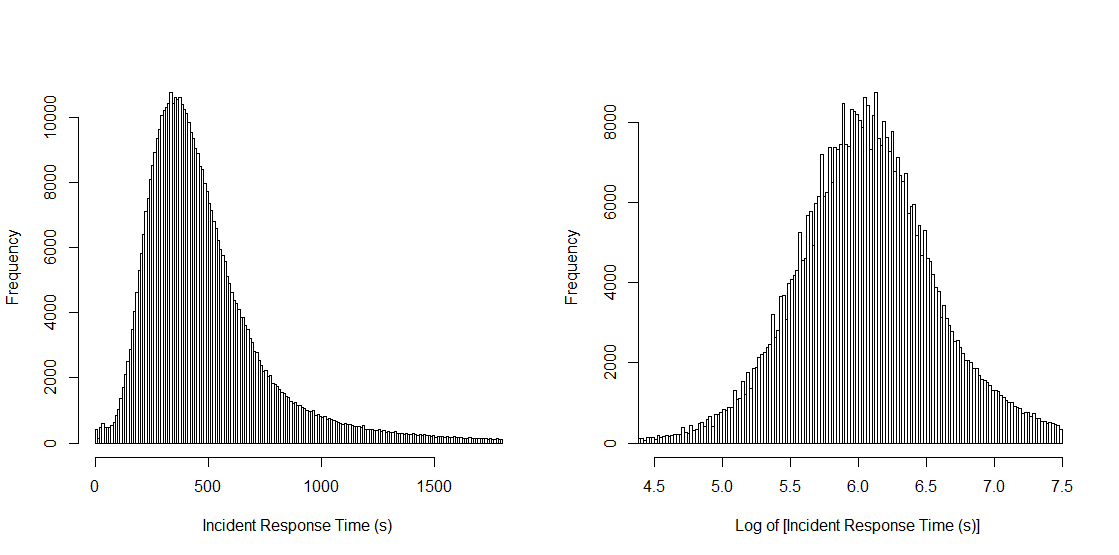
\includegraphics[width = 0.95\textwidth]{hist1.png}
    \caption{Histogram of Y variable}
    \label{fig:my_label}
\end{figure}

\begin{figure}
    \centering
    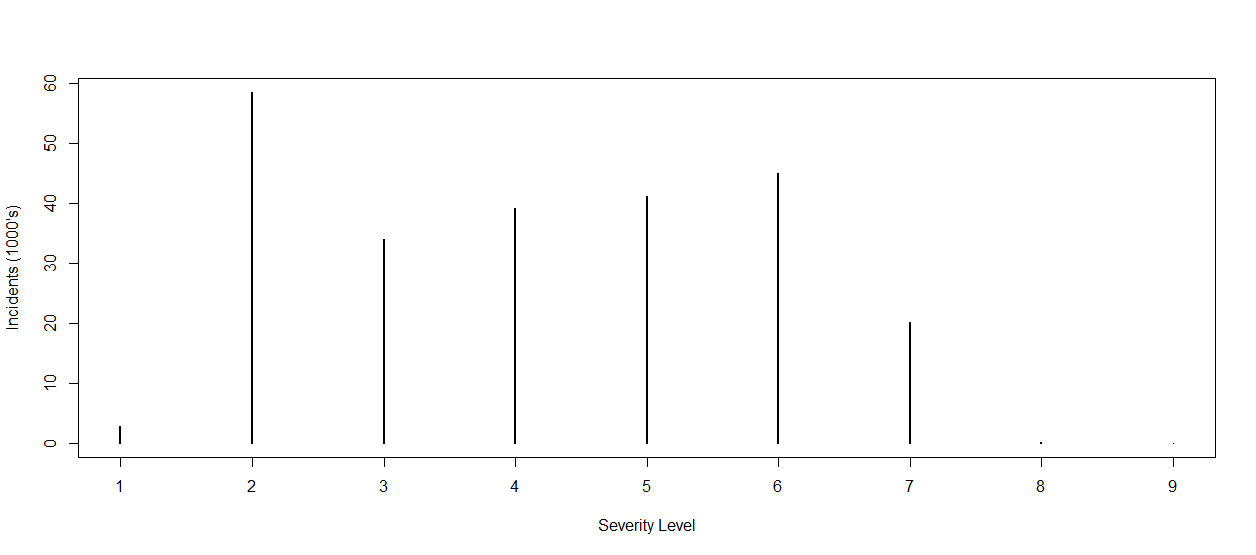
\includegraphics[width = 0.95\textwidth]{severity.png}
    \caption{Distribution of Initial Severity Levels}
\end{figure}

\begin{table}[H]
\centering
\begin{tabular}{rr}
  \hline
 & \% of Calls \\ 
  \hline
BRONX & 24.42 \\ 
  BROOKLYN & 29.20 \\ 
  MANHATTAN & 23.07 \\ 
  QUEENS & 19.13 \\ 
  RICHMOND / STATEN ISLAND & 4.18 \\ 
   \hline
\end{tabular}
\caption{\% of Reports, by Borough} 
\end{table}


\subsection{Data Extraction}

Several datasets were combined and filtered (based on some assumptions) to develop the dataset for this project. First, while \emph{NYC Open Data} provides EMS Data for the last five years, we filtered out data for only the last full year available - 2016. Next, we used the "Response Time" Boolean variable from the raw data, to filter out all entries for which there was no valid response time. We also filtered out entries where the value of the regressand variable (i.e. "INCIDENT\_RESPONSE\_TIME"  were  either 0 (this is likely indicative of no response, or a data entry error), or greater than 30 minutes (this covered over 95\% of all raw data, and we believe that times of greater than half an hour are outliers). There were a limited number of rows with missing data for the variables we intended to use for our predictive model, so we simply stripped those rows out as well. As a last step, we randomly divided the raw data into three sections - 50\% for developing out models, 30\%  for tuning, and 20\% for final prediction tests.

\subsection{Feature Choices}

As discussed, the primary aim of this project is to predict response time as soon as first contact is made with a caller. Therefore, even though the data contains a myriad information  that would have been collected after the first responders have arrived on the scene (such as "Final Recorded Severity Code", "Hospitalization (Y/N)"), we did not use this in our project. Our first linear model included the following information from the EMS dataset that we believe would be available as soon as the call is placed:
\begin{enumerate}
    \item Time of Day
    \item Month
    \item Initial Call Severity Level: From 1-9 as assigned by the EMS call center based on the description of the caller's problem.
    \item The Borough (one of five boroughs in NYC)
    \item ZIP Code from which the call was placed (as a FACTOR, not INTEGER type variable)
    \item Demographic data for the ZIP Code (\% gender distribution, \% race  distribution, \% on SNAP/government assistance, etc), from the 2010 US Census.
    \item Incident Travel Time: the time in seconds that the EMS vehicle takes to travel to the destination (this is, strictly speaking, not something that we can have access to at first call, but was included in the first model to evaluate its ability to make predictions).
\end{enumerate}

It must be noted here, that for "Time of Day" and "Month", a cosine transform was used to make the variables cyclical between 0 and 1. Furthermore, as is clear from the histogram in Figure 1, the Y-Variable appears to mimic a logarithmic distribution - so a log transform of this variable was used for the model.

Upon building the first linear regression model, we saw that the "Travel Time" was the strongest predictor of response time, which impedes a model's actual usability in the intended manner. Therefore, for subsequent models, we did not use this feature at all.  Figure 3 shows the apparent strong dependency between travel time and response time.
\begin{figure}
    \centering
    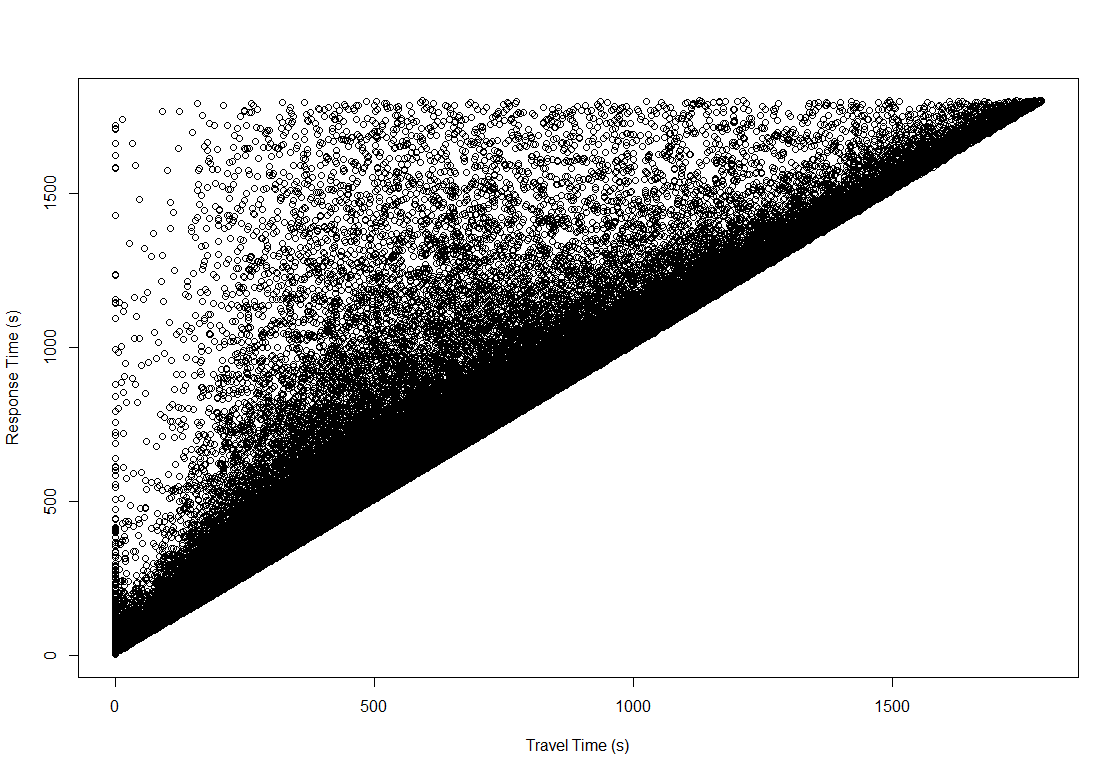
\includegraphics[width = 0.95\textwidth]{traveltime.png}
    \caption{Response Time as a Function of Travel Time}
\end{figure}


\subsection{Comparison \& Evaluation Methods}
The models discussed were compared to each other using the root-mean-square of error of predictions on the tuning and testing datasets, since all the models (including the neural net) were set to work as linear regressors.

\section{Method}
The machine learning models used for this project were built in \textbf{R} and the code can be found on my public \href{https://github.com/acharyaprithvi/90904-project/blob/master/final_project_code.rmd}{Github repository}.

We built the following model:

\subsection{Model 1: Linear Regression Model  With all Features}
Here, we used the \emph{lm} package that is a part of base R, to develop a linear regression model with all the regressors discussed in Section 3.3. On the 50\% training set, the model displayed an R-squared value of 0.93, and the variable importance of the few most important variables are presented in Table 4, in Appendix II. The variable importances were calculated using the \emph{VarImp} function in the \textbf{caret} package. Clearly, we see here, that the Travel Time variable is by far the most important regressor, and as discussed earlier, an ideal model for predicting response time at the time of first call should not include this regressor. Therefore, we built a second linear regression model, all the same regressors as Model 1, except for the Travel Time regressor, which we removed. It is also interesting to observe in  Table 4, that none of the demographic variables were deemed to be important at all in the regression model. Therefore, we built a third model, where we used neither the travel time, nor the demographic variables.


\subsection{Model 2: Linear Model without Travel Time}

When we excluded the "travel time" variable, we can see that the most important variables were the severity level, and the locations. Surprisingly, the month of the year was far more important than the time of day (which was not all that important). This model appears to be of substantially lower quality than the first model, however, with a much lower R-squared value (Table 5, Appendix II).


\subsection{Model 3: Linear Model with neither Travel Time nor Demographic Variables}
Since we observed that the demographic variables had no importance at all, we built a third model without these variables, and compared the predictive performance of our first three linear models over the tuning set. The results were as described below in Table 3.

\begin{table}[H]
\centering
\begin{tabular}{lll}
  \hline
Model & rMSE \\ 
  \hline
Model 1 & 0.139 \\ 
Model 2 & 0.504 \\ 
Model 3 & 0.503 \\ 
   \hline
\end{tabular}
\caption{Comparing Linear Models} 
\end{table}

Clearly from these results in Table 3, the model performs significantly better with the Travel Time variable than without, and the variables for demographics have little bearing. The next two models we built had the same regressors as Model 2, but used ensemble models instead of simply a single linear model.

\subsection{Model 4: Random Forest}
We used the \textbf{randomForest}  package to build a 50-tree  ensemble random forest model using the same regressors as Model 2. Figure 4 shows the improved performance of the ensemble with the increase in number of trees. Based on the leveling off  towards the bottom of this plot, the marginal benefit of increasing the number of trees is likely quite small. On our tuning dataset, the  Random Forest predicted with an rMSE of 0.252, which is a substantial improvement over the linear Model 2, but still not as good a predictor as the model with the Travel Time.

\begin{figure}
    \centering
    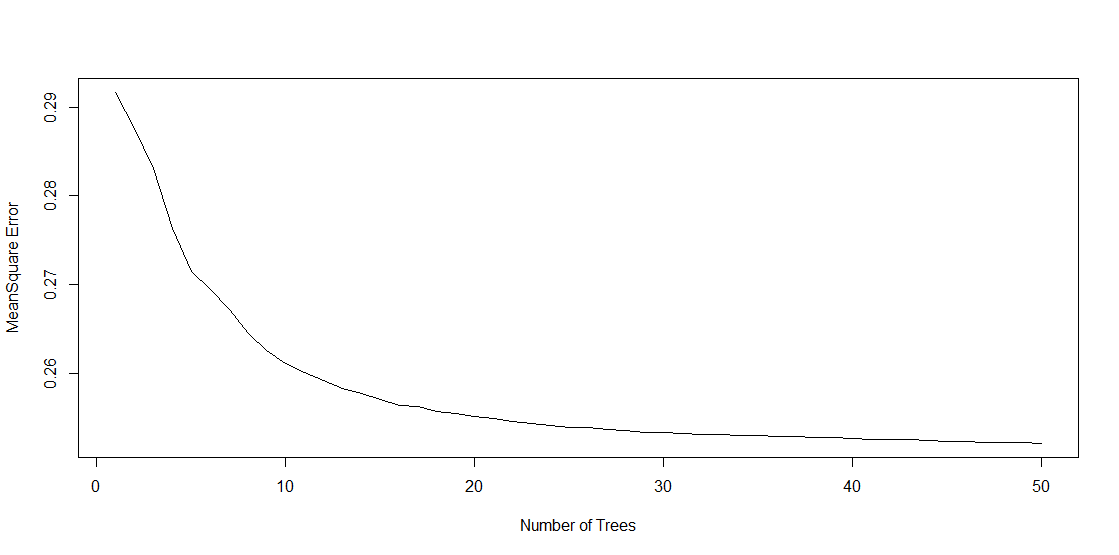
\includegraphics[width = 0.95\textwidth]{randfor.png}
    \caption{Random Forest Ensemble Performance}
\end{figure}


\subsection{Model 5: Neural Network}

We built a neural network using the \textbf{NN} R-package, with all the integer/numeric type regressors from Model 2, having two hidden nodes. The resulting network model is shown in Appendix I. This model performed rather poorly, with an rMSE in excess of 1.2.  

\section{Results}

Based on model performance from the tuning set, we retrained models 1, 2, and 4 with data from the existing training and tuning sets, and then used these new models to predict on the final 20\% data-set. As we can see, neither of Models 2 and 4 performed particularly well.

\begin{table}[H]
\centering
\begin{tabular}{rll}
  \hline
 Model & rMSE \\ 
  \hline
Model 1 & 0.1393 \\ 
Model 2 & 0.5041 \\ 
Model 3 & 0.4887 \\ 
   \hline
\end{tabular}
\caption{rMSE of Prediction on Final 20\%} 
\end{table}

\begin{figure}
    \centering
    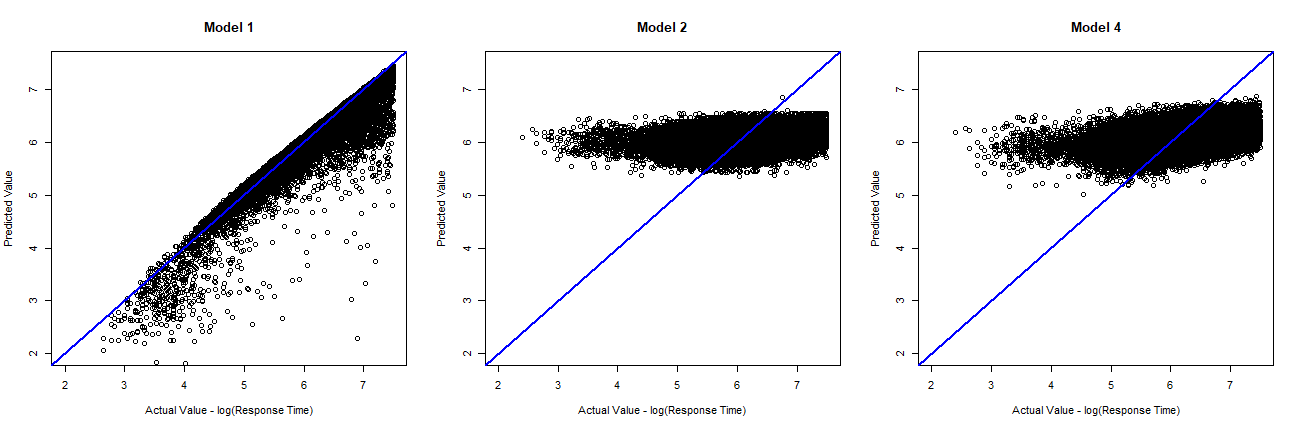
\includegraphics[width = 1.1\textwidth]{preds.png}
    \caption{Final Model Predictions}
\end{figure}


\section{Conclusion}
It would appear that the "travel time" is the only really strong predictor of response time, and that most other variables (such as the ZIP Code, time of day, or demographic variables) are either unimportant, or highly correlated with travel time so as to not matter to a model. Given our initially stated aim, the \textbf{Random Forest Ensemble Model} we developed is likely the best method to predict the expected response time, when the first call is received. \emph{However,}, as can be seen in Figure 5, any model without the "travel time" as a regressor is a relatively bad predictor. Therefore, future work will to enhance these models and make them usable will likely hinge heavily on collecting data related to :
* traffic,
* availability of ambulances,
* density of ambulances in a particular area, etc.,
which we can then use to build a model to first predict the travel time (several algorithms for point-to-point travel time estimates already exist), and then use that model to feed into an ensemble that can predict response time.


\newpage
\section*{Appendix I: Descriptive Statistics}

\setlength{\tabcolsep}{1pt}
\begin{table}[H]
\centering
\begin{tabular}{lllll}
  \hline
 & Min & Median & Mean & Max \\ 
  \hline
INITIAL\_SEVERITY\_LEVEL\_CODE & Min.   :1.0   & Median :4.0   & Mean   :4.135   & Max.   :9.0   \\ 
  FINAL\_SEVERITY\_LEVEL\_CODE & Min.   :1.0   & Median :4.0   & Mean   :4.015   & Max.   :8.0   \\ 
  DISPATCH\_RESPONSE\_SECONDS\_QY & Min.   :   1.00   & Median :  25.00   & Mean   :  43.98   & Max.   :1725.00   \\ 
  INCIDENT\_RESPONSE\_SECONDS\_QY & Min.   :   1.0   & Median : 422.0   & Mean   : 482.2   & Max.   :1800.0   \\ 
  INCIDENT\_TRAVEL\_TM\_SECONDS\_QY & Min.   :   0.0   & Median : 386.0   & Mean   : 438.2   & Max.   :1789.0   \\ 
  PERCENT.FEMALE & Min.   :0.00   & Median :0.4300   & Mean   :0.3609   & Max.   :1.00   \\ 
   PERCENT.MALE & Min.   :0.00   & Median :0.2600   & Mean   :0.2638   & Max.   :1.00   \\ 
  PERCENT.PACIFIC.ISLANDER & Min.   :0.0   & Median :0.0   & Mean   :0.03387   & Max.   :0.02000   \\ 
  PERCENT.HISPANIC.LATINO & Min.   :0.00   & Median :0.00   & Mean   :0.1591   & Max.   :1.00   \\ 
  PERCENT.AMERICAN.INDIAN & Min.   :0.00   & Median :0.00   & Mean   :0.004621   & Max.   :0.2000   \\ 
  PERCENT.ASIAN.NON.HISPANIC & Min.   :0.0   & Median :0.0   & Mean   :0.08539   & Max.   :1.0   \\ 
  PERCENT.WHITE.NON.HISPANIC & Min.   :0.00   & Median :0.00   & Mean   :0.1229   & Max.   :1.00   \\ 
  PERCENT.BLACK.NON.HISPANIC & Min.   :0.00   & Median :0.00   & Mean   :0.2103   & Max.   :1.00   \\ 
  PERCENT.OTHER.ETHNICITY & Min.   :0.0   & Median :0.0   & Mean   :0.03674   & Max.   :0.500   \\ 
  PERCENT.ETHNICITY.UNKNOWN & Min.   :0.0   & Median :0.0   & Mean   :0.00513   & Max.   :0.250   \\ 
  PERCENT.PERMANENT.RESIDENT.ALIEN & Min.   :0.0   & Median :0.0   & Mean   :0.04027   & Max.   :1.0   \\ 
  PERCENT.US.CITIZEN & Min.   :0.00   & Median :0.90   & Mean   :0.5796   & Max.   :1.00   \\ 
  PERCENT.RECEIVES.PUBLIC.ASSISTANCE & Min.   :0.00   & Median :0.0600   & Mean   :0.1861   & Max.   :1.00   \\ 
  PERCENT.NRECEIVES.PUBLIC.ASSISTANCE & Min.   :0.00   & Median :0.5500   & Mean   :0.4386   & Max.   :1.00   \\ 
   \hline
\end{tabular}
\caption{Descriptive Statistics} 
\end{table}
\setlength{\tabcolsep}{5pt}
\newpage
\section*{Appendix II: Linear Model Variable Importance}

\begin{table}[H]
\centering
\begin{tabular}{rlr}
  \hline
 & Parameter & Score \\ 
  \hline
1 & log(INCIDENT\_TRAVEL\_TM\_SECONDS\_QY) & 1692.554 \\ 
  2 & INITIAL\_SEVERITY\_LEVEL\_CODE & 70.699 \\ 
  3 & TIME\_OF\_DAY & 10.365 \\ 
  4 & BOROUGHRICHMOND / STATEN ISLAND & 6.717 \\ 
  5 & ZIPCODE10021 & 5.552 \\ 
  6 & ZIPCODE10034 & 5.244 \\ 
  7 & BOROUGHQUEENS & 0.828 \\ 
  8 & BOROUGHBROOKLYN & 0.447 \\ 
   \hline
\end{tabular}
\caption{First Model, Variable Importance Scores} 
\end{table}

\begin{table}[H]
\centering
\begin{tabular}{llr}
  \hline
 & Parameter & Score \\ 
  \hline
1 & INITIAL\_SEVERITY\_LEVEL\_CODE & 131.44 \\ 
  2 & ZIPCODE11101 & 22.36 \\ 
  3 & ZIPCODE11433 & 20.08 \\ 
  4 & ZIPCODE11370 & 20.07 \\ 
  5 & BOROUGHQUEENS & 19.07 \\ 
  6 & MONTH & 13.58 \\ 
  7 & BOROUGHRICHMOND / STATEN ISLAND & 8.80 \\ 
  8 & BOROUGHMANHATTAN & 7.27 \\ 
  9 & BOROUGHBROOKLYN & 3.71 \\ 
  10 & TIME\_OF\_DAY & 0.19 \\ 
   \hline
\end{tabular}
\caption{Model 2: Variable Importance} 
\end{table}


\newpage

\section*{Appendix III: Neural Network}

\begin{figure}[H]
    \centering
    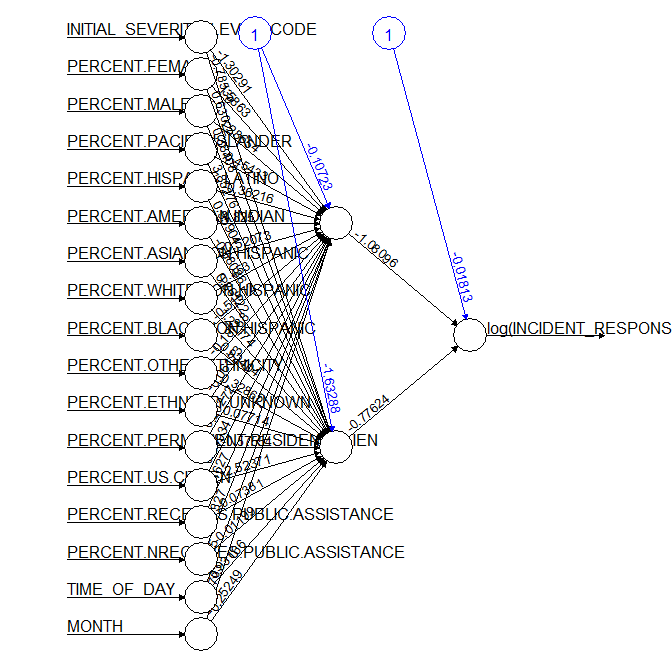
\includegraphics[width = 0.85\textwidth]{neuralnet.png}
    \caption{Neural Network}
\end{figure}


\newpage
\printbibliography
%\appendix
%\section*{Appendix A.}
%Some more details about those methods, so we can actually reproduce them.

\end{document}
